\documentclass{article}
\usepackage{iclr2027_conference,times}

\usepackage{amsmath,amssymb,amsthm}
\usepackage{booktabs}
\usepackage{multirow}
\usepackage{graphicx}
\usepackage{capt-of}
\usepackage{microtype}
\usepackage{xcolor}
\usepackage{tikz}
\usetikzlibrary{arrows.meta,positioning}
\usepackage[colorlinks=true,linkcolor=blue,citecolor=blue]{hyperref}
\usepackage{url}
\usepackage{algorithm}
\usepackage{algpseudocode}

% ----------------------------------------------------------------------
% Macros
% ----------------------------------------------------------------------

\newcommand{\E}{\mathbb{E}}
\newcommand{\ind}[1]{\mathbf{1}\!\left[#1\right]}
\newcommand{\sg}{\mathrm{sg}}
\newcommand{\cube}{c}
\newcommand{\Reach}{\mathrm{reach}}
\newcommand{\Visit}{\mathrm{visit}}
\newcommand{\TDFB}{\textsc{TDFB}}
\newcommand{\DensityFB}{\textsc{Density-FB}}

\newtheorem{proposition}{Proposition}

\title{Learning Successor Measures from Manipulation Play}
\author{Anonymous}

% \iclrfinalcopy

\begin{document}
\maketitle

% ======================================================================
\section{Preliminaries}
\label{sec:prelim}

\paragraph{Successor measures.}
We consider a Markov decision process with state space $\mathcal S$, action space $\mathcal A$, transition kernel $P$, and discount factor $\gamma\in(0,1)$.
The successor measure of a policy $\pi$ is its discounted future-state occupancy:
\begin{equation}
\label{eq:sm}
M^\pi(s,a,X) = \E_\pi\!\left[ \sum_{t\ge0}\gamma^t \ind{s_{t+1}\in X} \;\middle|\; s_0=s,a_0=a \right].
\end{equation}
For any reward $r$, the corresponding action value is
\begin{equation}
\label{eq:q-from-sm}
Q_r^\pi(s,a) = \int r(x)\,dM^\pi(s,a,x).
\end{equation}
Successor measures therefore separate learning future dynamics from specifying the downstream reward \citep{dayan1993improving,blier2021learning}.

Their Bellman equation is
\begin{equation}
\label{eq:sm-bellman}
M^{\pi_z}(s,a,X) = P(s'\in X\mid s,a) + \gamma \E_{s',a'\sim\pi_z} \left[ M^{\pi_z}(s',a',X) \right].
\end{equation}


\paragraph{Forward-backward representations.}
Forward-backward representations \citep{touati2021learning,touati2023does} factorize the density of the successor measure with respect to a reference distribution $\rho$, typically the dataset marginal:
\begin{equation}
\label{eq:fb}
M^{\pi_z}(s,a,X) \approx \int_X F(s,a,z)^\top B(x)\,d\rho(x).
\end{equation}
The forward representation $F(s,a,z)$ describes occupancy induced by policy $\pi_z$, while $B(x)$ embeds an independently queried future state.

For a new reward,
\begin{equation}
\label{eq:fb-z}
z_r \propto \E_{x\sim\rho} \left[ r(x)B(x) \right],
\end{equation}
and FB evaluates it as
\begin{equation}
\label{eq:fb-q}
Q_r(s,a) \approx F(s,a,z_r)^\top z_r.
\end{equation}
One learned representation can therefore support many rewards without learning a new value function.


\paragraph{Scalar FB objective.}
Let
\begin{equation}
m_z(s,a,x) = F(s,a,z)^\top B(x).
\end{equation}
Standard FB uses the surrogate
\begin{equation}
\label{eq:fb-loss}
\mathcal L_{\mathrm{FB}} = \frac12 \E_{x\sim\rho} \left[ (m_z-\gamma\bar m_z)^2 \right] - \E \left[ m_z(s,a,s') - \gamma\bar m_z(s,a,s') \right] + \lambda_{\mathrm{ortho}} \mathcal L_{\mathrm{ortho}}.
\end{equation}
Random query states receive a squared residual, while the observed successor receives a linear positive term.


% ======================================================================
\section{Manipulation play separates transitions from persistent outcomes}
\label{sec:play}

\subsection{Objects move briefly and rest for long periods}
\label{sec:dwell}

In locomotion and maze navigation, the variable used to specify the task is usually the agent's own position or configuration.
As the agent acts, it also moves through goal space.

Manipulation play has a different structure.
The robot may approach an object, grasp it, transport it, release it, and continue acting while the object remains fixed.
The full state therefore continues to change even when the task-relevant object configuration does not.

A typical play sequence has the form
\[ \underbrace{ \text{approach} \rightarrow \text{grasp} \rightarrow \text{transport} \rightarrow \text{release} }_{\text{object-changing interaction}} \rightarrow \underbrace{ \text{rest} \rightarrow \text{rest} \rightarrow \cdots }_{\text{persistent outcome}}. \]

This persistence is substantial in OGBench.
On \texttt{cube-single-play-v0}, cube position is unchanged on $48\%$ of transitions and stationary runs have median length $44$ steps.
A $4$\,cm region around a random dataset state contains only $1.3\%$ of the data, yet after entering such a region a trajectory accumulates approximately $25$--$31$ discounted visits there.
On \texttt{cube-double-play-v0}, each cube is stationary on $72\%$ of transitions.
On \texttt{scene-play-v0}, the drawer and window are stationary on $91\%$ of transitions and buttons on $99.6\%$.

\begin{figure}[t]
\centering
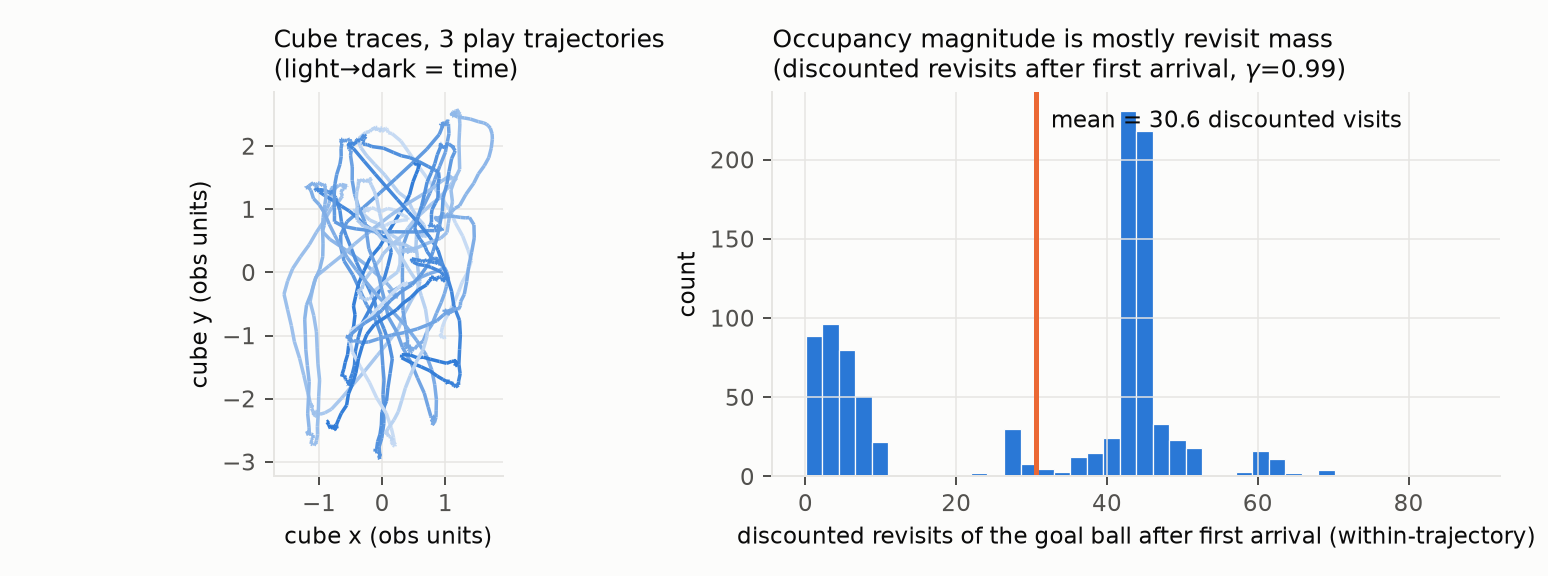
\includegraphics[width=0.95\textwidth]{figures/playdata.png}
\caption{Manipulation play alternates between brief object-changing interactions and long periods at persistent configurations. \emph{Left:} three \texttt{cube-single} play trajectories. \emph{Right:} discounted occupancy accumulated after first entering a $4$\,cm goal region. Most of the successor mass is accumulated after arrival.}
\label{fig:playdata}
\end{figure}


\subsection{The successor measure contains two very different signals}
\label{sec:reach-vs-visit}

Let $\cube(s)$ denote the object configuration and define a goal region
\begin{equation}
B_\epsilon(g) = \left\{ s: \|\cube(s)-\cube(g)\| \le\epsilon \right\},
\end{equation}
with indicator
\begin{equation}
h(s',g) = \ind{s'\in B_\epsilon(g)}.
\end{equation}

The discounted occupancy of this region is
\begin{equation}
\label{eq:visit}
M^{\Visit}(s,a,g) = \E_\pi \left[ \sum_{t\ge0} \gamma^t h(s_{t+1},g) \right].
\end{equation}

Let
\begin{equation}
T_g = \min \left\{ t\ge0: s_{t+1}\in B_\epsilon(g) \right\}
\end{equation}
be the first hitting time.
Then
\begin{align}
M^{\Visit}(s,a,g) &= \underbrace{ \E_\pi \left[ \gamma^{T_g} \ind{T_g<\infty} \right] }_{Q^{\Reach}(s,a,g)} \nonumber\\ &\quad+ \underbrace{ \E_\pi \left[ \ind{T_g<\infty} \sum_{t>T_g} \gamma^t h(s_{t+1},g) \right] }_{\text{post-arrival occupancy}}.
\label{eq:decomp}
\end{align}

The first term measures whether an action eventually reaches the goal and how quickly.
The second measures what happens after arrival.

These terms play different roles in manipulation.
Goal-reaching evaluation depends primarily on the first.
General reward transfer requires both.

On play data, however, the second term is numerically much larger.
A regressor given only the goal predicts post-arrival occupancy with Spearman correlation $0.60$--$0.63$, whereas the reachability value predicts it at only $0.06$.
Thus much of the successor measure's magnitude describes where objects persist, while the action differences needed for reaching live in a smaller component.


\subsection{Why this stresses scalar FB}
\label{sec:scalar-failure}

The successor measure itself remains the correct object.
The difficulty is estimating it with a finite-capacity scalar factorization.

During a long resting segment, many different robot states and actions correspond to nearly the same object configuration:
\[ (s_1,a_1), (s_2,a_2), \ldots, (s_L,a_L) \quad\longrightarrow\quad \cube(s_t)\approx x_{\mathrm{rest}}. \]
These transitions legitimately contribute large successor mass near $x_{\mathrm{rest}}$.
But they provide much less information about which earlier actions caused the object to arrive there.

Standard FB compounds this imbalance.
Its observed-successor term is linear in the matched score, so repeated successors continually reward larger values of $F^\top B$ at persistent configurations.
The model must therefore recover small action-dependent differences inside a much larger occupancy signal.

This issue is distinct from the formal singularity of point densities under deterministic continuous dynamics.
That singularity is also present in locomotion domains where FB performs well.
Our hypothesis is instead that manipulation play makes the scalar estimation problem practically difficult because persistent outcomes dominate the sampled occupancy distribution.


% ======================================================================
\section{Successor learning from manipulation play}
\label{sec:methods}

We study two responses to the same data structure.

\TDFB{} first learns the action-sensitive reaching signal and only then restores full occupancy.
\DensityFB{} instead learns the complete successor measure from the beginning, but represents it as a normalized probability distribution so persistent occupancy cannot increase the model's total scale.


% ----------------------------------------------------------------------
\subsection{\TDFB: learn reaching before occupancy}
\label{sec:tdfb}

\TDFB{} replaces exact-state queries with finite object-space regions and uses bounded TD targets while retaining the FB factorization
\begin{equation}
\label{eq:tdfb-factor}
M_\theta(s,a,z,g) = F_\theta(s,a,z)^\top B_\phi(g).
\end{equation}

For a transition $(s,a,s')$ and goal $g$,
\begin{equation}
h(s',g) = \ind{ \|\cube(s')-\cube(g)\| \le\epsilon } \in\{0,1\}.
\end{equation}


\paragraph{Phase 1: reaching.}
We first learn
\begin{equation}
\label{eq:reach}
Q^{\Reach}(s,a,g) = \E \left[ \gamma^{T_g} \ind{T_g<\infty} \right],
\end{equation}
using the absorbing target
\begin{equation}
\label{eq:reach-target}
y^{\Reach} = h + \gamma(1-h) \bar Q^{\Reach} \left( s', \pi_{\bar\omega}(s',z_g), g \right).
\end{equation}

The factor $(1-h)$ stops the backup after the first hit.
A trajectory
\[ \text{approach} \rightarrow \text{grasp} \rightarrow \text{transport} \rightarrow \text{hit} \rightarrow \text{rest} \rightarrow\cdots \]
therefore contributes only through the first arrival.
The representation is forced to distinguish the actions responsible for reaching the object configuration rather than repeatedly fitting what happens after success.


\paragraph{Phase 2: occupancy.}
We then initialize from Phase 1, freeze the backward representation, and learn the non-absorbing target
\begin{equation}
\label{eq:visit-target}
y^{\Visit} = h + \gamma \bar M^{\Visit} \left( s', \pi_{\bar\omega}(s',z), z, g \right).
\end{equation}
Its fixed point is the full region successor measure,
\begin{equation}
M^{\Visit}(s,a,z,g) = \E_{\pi_z} \left[ \sum_{t\ge0} \gamma^t h(s_{t+1},g) \right].
\end{equation}

The two phases therefore implement a curriculum: first learn which actions produce object outcomes, then learn how long those outcomes are occupied.

\paragraph{Limitation.}
Region grounding becomes sparse in joint object space.
On \texttt{cube-double}, a randomly sampled conjunctive goal gives a positive region target on only $0.046\%$ of state-goal pairs.
Hindsight queries improve this signal, but without importance correction they change the query distribution defining the learned measure.


% ----------------------------------------------------------------------
\subsection{\DensityFB: learn normalized occupancy directly}
\label{sec:densityfb}

\DensityFB{} removes the need for a reaching curriculum by changing the parameterization of the successor measure itself.

\paragraph{Normalize the measure.}
For object coordinates $x=\phi_{\mathrm{obj}}(s)$, define
\begin{equation}
M(\cdot\mid s,a,g) = \E \left[ \sum_{t\ge0} \gamma^t \delta_{x_{t+1}} \right].
\end{equation}
Its total mass is always
\begin{equation}
M(\mathcal X\mid s,a,g) = \frac{1}{1-\gamma}.
\end{equation}
Therefore
\begin{equation}
\label{eq:nu}
\nu(\cdot\mid s,a,g) = (1-\gamma) M(\cdot\mid s,a,g)
\end{equation}
is a probability measure.
$M$ and $\nu$ contain exactly the same information.


\paragraph{Retain the FB two-tower representation.}
Rather than interpreting a dot product directly as occupancy, we use it as a score:
\begin{equation}
\label{eq:density-score}
f(s,a,g,u) = F_\theta(s,a,g)^\top B_\phi(\tilde u) /\tau,
\end{equation}
where $\tilde u$ denotes appropriately scaled object coordinates.

For a query set
\begin{equation}
U=\{u_j\}_{j=1}^K,
\end{equation}
the predicted normalized occupancy is
\begin{equation}
\label{eq:density-softmax}
w_j(s,a,g) = \frac{ \exp f(s,a,g,u_j) }{ \sum_{k=1}^K \exp f(s,a,g,u_k) }.
\end{equation}

Thus
\begin{equation}
w_j\ge0, \qquad \sum_jw_j=1.
\end{equation}
Non-negativity and total mass are properties of the parameterization rather than auxiliary penalties.


\paragraph{Queries are resampled.}
The query set $U$ is redrawn from the object-state marginal at every update.
The number of queries is therefore a Monte-Carlo sample count rather than a fixed discretization of object space.
The checkpoint retains only the continuous functions $F$ and $B$.


\paragraph{Distributional Bellman learning.}
Let $\kappa(\cdot\mid x')$ be a normalized kernel around the observed next object configuration.
The normalized successor Bellman target is
\begin{equation}
\label{eq:density-target}
t = \sg \left[ (1-\gamma) \kappa(\cdot\mid x') + \gamma \bar p(s',a^+,g) \right],
\end{equation}
where
\begin{equation}
a^+ \sim \pi_{\bar\omega}(\cdot\mid s',g).
\end{equation}

Both terms lie on the simplex, and their coefficients sum to one.
We therefore fit the target using cross-entropy:
\begin{equation}
\label{eq:density-loss}
\mathcal L_{\mathrm{density}} = - \E \left[ \sum_j t_j \log w_j \right].
\end{equation}

Every transition supplies a complete distributional target.
This avoids the sparse conjunctive indicator required by \TDFB{} on multi-object tasks.


\paragraph{Why normalization matters on play.}
Persistent configurations should receive large successor mass.
\DensityFB{} does not remove this mass.
Instead, it forces all configurations to compete for a fixed total amount of probability.

Repeated observations of a resting configuration can therefore make the predicted distribution increasingly concentrated there, but cannot increase the total magnitude of the critic without bound.
The analogous action-independent solution is a broad or uniform distribution, which is penalized by cross-entropy whenever the Bellman target is concentrated.


\paragraph{Control.}
For a goal $g$, the actor maximizes the predicted occupancy of its neighborhood:
\begin{equation}
\label{eq:density-control}
q(s,a,g) = w(s,a,g)^\top \kappa(\cdot\mid g).
\end{equation}


\paragraph{Arbitrary rewards.}
For any reward $r$ evaluated on the query set,
\begin{equation}
\label{eq:density-readout}
\widehat Q_r(s,a) = \frac{ r(x_0) + \left( w-\kappa(\cdot\mid x_0) \right)^\top r(U) }{ 1-\gamma }.
\end{equation}
The value remains exactly linear in the downstream reward.


% ----------------------------------------------------------------------
\subsection{Two views of the same problem}
\label{sec:method-connection}

The two methods differ in how they handle persistent occupancy.

\begin{center}
\begin{tabular}{p{0.21\textwidth}p{0.34\textwidth}p{0.34\textwidth}}
\toprule
& \TDFB{} & \DensityFB{} \\
\midrule
What is learned first? & First-arrival value & Full successor measure \\
How is dwell handled? & Ignored during Phase 1, restored in Phase 2 & Retained from the start, but normalized \\
Immediate grounding & Binary region event & Distribution around observed successor \\
Multi-object issue & Conjunctive region events become sparse & Every joint successor supplies a target \\
Successor-measure readout & Region approximation & Continuous Monte-Carlo integration \\
\bottomrule
\end{tabular}
\end{center}

Both methods exploit the same observation: play contains comparatively brief action-sensitive object transitions and long periods of persistent object occupancy.
\TDFB{} first isolates the former.
\DensityFB{} learns both together under a parameterization in which the latter cannot dominate the scale of the estimator.


% ======================================================================
\section{Experiments}
\label{sec:experiments}

\paragraph{Environments.}
We use OGBench state-based manipulation \citep{park2024ogbench}.
Our main environments are \texttt{cube-single-play-v0}, \texttt{cube-double-play-v0}, and \texttt{scene-play-v0}.
No benchmark reward labels are used to train the successor representations.

\paragraph{Protocol.}
Unless stated otherwise, models train for $500$k gradient steps.
Goal-conditioned success is measured using the environment's native evaluation over five tasks and $50$ episodes per task.
Reported \DensityFB{} results use three seeds.


% ----------------------------------------------------------------------
\subsection{Successor learning can recover manipulation from play}
\label{sec:main-results}

Table~\ref{tab:main} reports goal-conditioned success.

\begin{table}[t]
\centering
\small
\setlength{\tabcolsep}{5pt}
\begin{tabular}{lccc}
\toprule
Method & \texttt{cube-single} & \texttt{cube-double} & \texttt{scene} \\
\midrule
Behavior cloning & $0.111$ & $0.019$ & --- \\
Plain FB & $0.420$ & $0.000$ & $0.047$ \\
Goal-conditioned IQL & $0.879$ & $0.265$ & $0.26$--$0.287$ \\
\midrule
\TDFB{} reachability & $\mathbf{0.967}$ & $0.549$ & $0.484$ \\
\TDFB{} occupancy, dataset queries & $0.952$ & $0.358$ & $0.342$ \\
\TDFB{} occupancy, hindsight queries & $\sim0.93$ & $\sim0.53$ & $\mathbf{0.927}$ \\
\midrule
Occupancy reward shaping & $0.739$ & $0.364$ & --- \\
\DensityFB{} & $0.929 \pm 0.028$ & $\mathbf{0.736 \pm 0.046}$ & $0.628 \pm 0.054$ \\
\bottomrule
\end{tabular}
\caption{Native goal-conditioned success on OGBench manipulation. \texttt{cube-double} is the most discriminative current environment: the behavior-cloning floor is $0.019$, plain FB fails, and \DensityFB{} reaches $0.736$. \DensityFB{} entries are mean $\pm$ s.d.\ over three seeds at the final ($500$k) evaluation (\texttt{cube-single} $.896/.928/.964$; \texttt{cube-double} $.680/.736/.792$). All rows in this table use the environment's native training-loop evaluation ($50$ episodes per task); the appendix Table~\ref{tab:multi} uses the separate zero-shot harness and its direct-GC pass, whose numbers differ slightly for the same checkpoints. The occupancy-reward-shaping row is the reward-scale $4.0$ arm (three seeds); other scales were screened at one seed only.}
\label{tab:main}
\end{table}


\paragraph{CubeSingle.}
Several methods perform well once the successor representation is properly grounded.
\TDFB{} increases success from $0.42$ for plain FB to $0.967$, while \DensityFB{} reaches $0.929$ from scratch.
This indicates that the FB representation class has sufficient capacity for single-object manipulation.


\paragraph{CubeDouble.}
The difference becomes much larger in joint object space.
\TDFB{} reachability reaches $0.549$, but fitting occupancy with dataset-sampled conjunctive regions reduces success to $0.358$.
Hindsight queries recover approximately $0.53$ by increasing positive goal coverage.
\DensityFB{} instead reaches $0.736$ without hindsight queries or a two-stage curriculum.
The behavior-cloning floor of $0.019$ indicates that the result is not explained by policy imitation alone.


\paragraph{Scene.}
\TDFB{} with hindsight queries reaches $0.927$; \DensityFB{} reaches $0.628 \pm 0.054$ ($0.672/0.568/0.644$ at $500$k).
The aggregate hides a per-task split that is consistent across all three seeds: the first three tasks are near solved (\texttt{open}, \texttt{unlock-and-lock}, \texttt{rearrange-medium} at $0.88$--$1.0$) while the two long-composition tasks fail (\texttt{put-in-drawer} at $0.02$--$0.48$, \texttt{rearrange-hard} at $0.0$--$0.02$).
\DensityFB{} therefore clears every non-hindsight arm on \texttt{scene} but does not replace hindsight grounding there; why the two composed-rearrangement tasks fail while \texttt{rearrange-medium} succeeds is an open question rather than an averaged-away detail.


% ----------------------------------------------------------------------
\subsection{The scalar FB estimator is the bottleneck}
\label{sec:frozen}

We next ask whether plain FB fails because its representation is insufficient or because of how the successor measure is estimated.

We freeze a backward representation from a checkpoint already supporting approximately $0.97$ task success and optimize the scalar FB density estimator on top of it.
Without orthonormalization, critic scale increases from approximately $154$ to $5.4\times10^4$ within $65$k steps, while mean task success decreases from $0.98$ to $0.42$ by $100$k steps.
Allowing the backward representation to train accelerates the collapse.
With orthonormalization, scale remains bounded but performance reaches only $0.225$.

\begin{figure}[t]
\centering
\begin{minipage}[t]{0.48\textwidth}
\centering
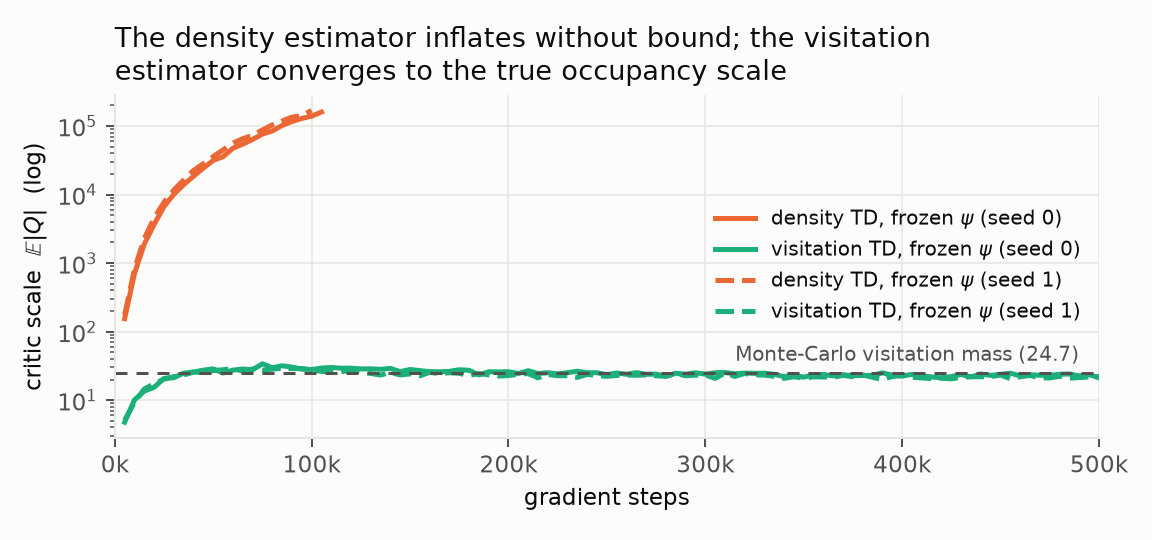
\includegraphics[width=\textwidth]{figures/scale_divergence.png}
\end{minipage}
\hfill
\begin{minipage}[t]{0.48\textwidth}
\centering
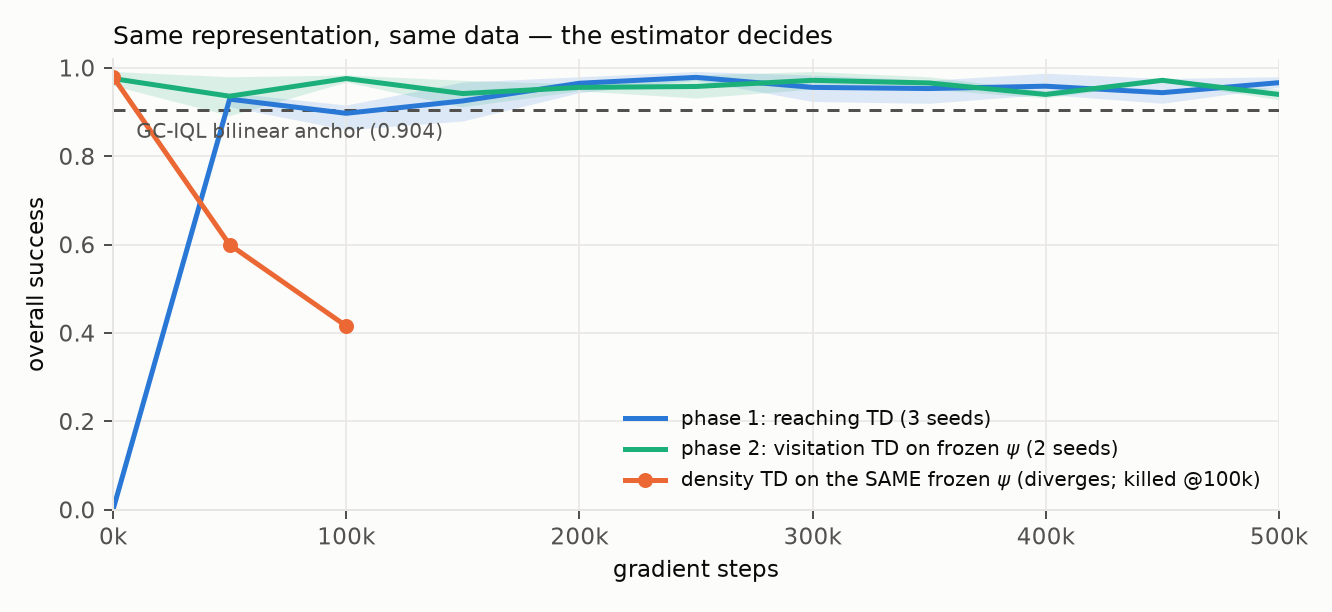
\includegraphics[width=\textwidth]{figures/2_curves.png}
\end{minipage}
\caption{A useful representation does not rescue the scalar FB objective. \emph{Left:} critic scale. \emph{Right:} goal-conditioned success. Bounded TD objectives remain stable, while the scalar FB density objective degrades even when the backward representation is frozen.}
\label{fig:divergence}
\end{figure}

These results rule out representation capacity as the sole explanation.
The same class of bilinear representations supports strong control under \TDFB{}, while the scalar FB estimator destabilizes it.


% ----------------------------------------------------------------------
\subsection{Why multi-object manipulation separates the methods}
\label{sec:multi}

The difference between the two methods is especially visible on \texttt{cube-double}.

Under \TDFB{}, a query goal requires both cubes to lie within their target regions.
With goals sampled from the dataset marginal, the immediate indicator is non-zero on only
\begin{equation}
4.6\times10^{-4}
\end{equation}
of state-goal pairs.
Changing kernel width, factorization rank, actor freezing, and their combinations does not remove the problem.
Hindsight queries help because they explicitly select reachable future joint configurations.

\DensityFB{} does not ask whether a transition matches one independently sampled conjunctive goal.
Every observed joint object configuration supplies a normalized target over the current continuous query set.
The method therefore retains dense grounding even as the dimensionality of the object configuration increases from three to six.


% ----------------------------------------------------------------------
\subsection{Measure quality}
\label{sec:measure-quality}

Strong control does not by itself establish that a model recovers the successor measure.
We therefore compare predicted set occupancy with Monte-Carlo rollouts.

For \DensityFB{}, coarse-scale ordering is strong: Spearman correlation reaches approximately $0.83$--$0.85$ at $4\epsilon$.
At the native $\epsilon$ scale, ordering is more moderate, approximately $0.41$--$0.48$.
Thus the current model recovers broad occupancy geometry more reliably than fine-grained set mass.

A symmetric comparison against the fixed-partition variant --- each method scored under its own deployed head aggregation --- gives partition Spearman of $0.778$--$0.790$ pooled, $0.423$--$0.477$ at native $\epsilon$, and $0.830$--$0.834$ at $4\epsilon$ across seeds, indistinguishable from \DensityFB{} ($0.767$--$0.789$ / $0.407$--$0.462$ / $0.831$--$0.848$).
The two parameterizations are calibration-equivalent at every scale; the control and transfer gains of the continuous support therefore do not come from a better-calibrated measure, and the native-$\epsilon$ weakness is a property of the estimator family rather than of either support.

The normalized parameterization nevertheless satisfies two properties structurally:
\begin{equation}
\nu(X)\ge0, \qquad \nu(\mathcal X)=1.
\end{equation}
Earlier scalar region estimators violated both properties without explicit regularization.


% ----------------------------------------------------------------------
\subsection{Reward transfer}
\label{sec:reward-transfer}

Goal-reaching evaluates only one use of a successor representation.
The motivation for successor measures is that one learned model should support many downstream rewards.

For \TDFB{}, occupancy fine-tuning improves reward transfer even when it slightly reduces goal-reaching success.
On \texttt{cube-single}, the mean held-out return increases from $16.8$ for the reachability representation to $20.3$ after occupancy training.
Adding reward-induced task embeddings and measure constraints raises this to $32.4$, compared with $17.2$ for the reimplemented FB baseline.

\begin{table}[t]
\centering
\small
\begin{tabular}{lcccc}
\toprule
Method & concentrated & broad & compositional & mean \\
\midrule
FB & $8.4$ & $35.4$ & $6.9$ & $17.2$ \\
\TDFB{} reachability & $12.1$ & $27.8$ & $8.5$ & $16.8$ \\
$+$ occupancy & $16.3$ & $28.5$ & $15.8$ & $20.3$ \\
$+$ reward-task coverage & $20.2$ & $31.5$ & $23.0$ & $24.5$ \\
$+$ measure constraints & $\mathbf{26.1}$ & $\mathbf{41.6}$ & $\mathbf{33.0}$ & $\mathbf{32.4}$ \\
\bottomrule
\end{tabular}
\caption{Held-out reward return on \texttt{cube-single}. The successor measure matters beyond first-passage control: occupancy learning substantially improves concentrated and compositional reward transfer.}
\label{tab:transfer}
\end{table}

\DensityFB{} admits the direct linear reward readout in Equation~\ref{eq:density-readout}.
A matched reward-transfer evaluation is ongoing.


% ======================================================================
\section{Related work}
\label{sec:related}

\paragraph{Successor representations and measures.}
Successor representations predict discounted future occupancy \citep{dayan1993improving}.
Successor measures extend this idea to continuous state spaces \citep{blier2021learning}.
Forward-backward representations factorize the successor density and learn a policy family that can be retargeted to downstream rewards \citep{touati2021learning,touati2023does}.
Our methods retain this reward-free occupancy perspective but study how the estimator interacts with persistent object configurations in manipulation play.


\paragraph{Goal-conditioned offline RL.}
Goal-reaching with sparse rewards and hindsight relabeling is standard in goal-conditioned RL \citep{kaelbling1993learning,andrychowicz2017hindsight,kostrikov2021offline,park2023hiql}.
\TDFB{} uses the corresponding first-passage value as an initialization for successor-measure learning rather than as the final representation.


\paragraph{Contrastive and distributional future-state learning.}
Contrastive RL \citep{eysenbach2022contrastive} learns future-state discrimination rather than an explicit unbounded successor density.
\DensityFB{} is also distributional but retains the FB policy-conditioned factorization and an explicit normalized successor-measure interpretation.


% ======================================================================
\section{Discussion}
\label{sec:discussion}

Our experiments point to a simple distinction between locomotion and manipulation play.
In locomotion, actions continuously change the variables used to specify downstream objectives.
In manipulation play, actions change objects during short interaction periods, while the resulting object configurations persist for long periods.

The successor measure correctly counts both.
The difficulty is that a finite-capacity estimator must preserve action-sensitive differences while fitting a signal whose magnitude is dominated by persistent outcomes.

\TDFB{} and \DensityFB{} address this issue differently.
\TDFB{} first learns a first-passage value, removing post-arrival occupancy from the initial representation, and then restores the complete successor measure.
\DensityFB{} retains the complete occupancy from the beginning but learns it as a probability distribution with fixed total mass.

The \texttt{cube-double} result favors the latter approach: normalization and dense continuous-query supervision avoid both the scalar-scale problem and the sparse conjunction problem that appears in region TD.
At the same time, \DensityFB{} on \texttt{scene} solves only three of the five tasks ($0.628$ aggregate vs $0.927$ for hindsight-grounded \TDFB{}), and fine-scale Monte-Carlo calibration remains weaker than coarse occupancy ordering.
Understanding these limitations is necessary before claiming a general manipulation behavior foundation model.


% ======================================================================
\section{Limitations}
\label{sec:limitations}

First, our methods are given the object coordinates used to define downstream goals.
Extending the same ideas to learned object representations from pixels is an important next step.

Second, \DensityFB{} currently uses each minibatch's next object configurations as its query set.
Whether independent replay queries give the same result, especially in sparse multi-object spaces, remains untested.

Third, \DensityFB{} recovers coarse occupancy ordering more reliably than occupancy at the smallest evaluated spatial scale.

Finally, on heterogeneous \texttt{scene} tasks Density-FB solves three of five tasks across all seeds while failing on the two composed-rearrangement tasks, suggesting that additional structure beyond simple geometric object coordinates may be required there; hindsight-grounded \TDFB{} remains the stronger method on that environment.


% ======================================================================
\bibliography{references}
\bibliographystyle{iclr2027_conference}


% ======================================================================
\appendix

\section{Additional play-data statistics}
\label{app:playstats}

On \texttt{cube-single-play-v0}, cube position satisfies
\begin{equation}
\|\Delta\cube\|<10^{-6}
\end{equation}
on $47.9\%$ of within-episode transitions.
Stationary runs have median length $44$ steps, mean $43.9$, and $90$th percentile $47$.

A $4$\,cm region around a random dataset state contains on average
\begin{equation}
\bar N=0.0137
\end{equation}
of the dataset.

Discounted occupancy accumulated after first arrival has mean approximately $24.7$ at the dataset level and approximately $30.6$ within trajectories.

For \texttt{cube-double-play-v0}, each cube is stationary on $72\%$ of transitions, both simultaneously on $48\%$, and the dataset-marginal mass of a random conjunctive region is
\begin{equation}
3.3\times10^{-4}.
\end{equation}
(This is the $\rho$-measure of the joint region itself; the $4.6\times10^{-4}$ quoted in Section~\ref{sec:multi} is the transition-level rate of non-zero immediate indicators over sampled state-goal pairs --- two related but distinct statistics.)
Post-arrival occupancy has mean $32.2$ and median $43$.

For \texttt{scene-play-v0}, the cube is stationary on $74\%$ of transitions, drawer and window on $91\%$, buttons on $99.6\%$, and all tracked variables simultaneously on $60\%$.
Post-arrival occupancy has mean $37.0$.


% ======================================================================
\section{Scalar FB divergence controls}
\label{app:fb-divergence}

The frozen-representation control uses a backward representation from a checkpoint supporting approximately $0.97$ goal-conditioned success.

\begin{itemize}
\item \textbf{Frozen $B$, scalar FB surrogate.} Critic scale grows from approximately $154$ to $5.4\times10^4$ within $65$k steps and success falls to approximately $0.42$ by $100$k steps.
\item \textbf{Trainable $B$, scalar FB surrogate.} Collapse is faster, reaching approximately $0.06$--$0.07$ success by $50$k steps.
\item \textbf{Frozen $B$, bounded indicator TD.} The critic converges to the Monte-Carlo occupancy scale and remains stable for $500$k updates.
\item \textbf{Scalar FB with orthonormalization.} Scale remains bounded but task success reaches only $0.225$.
\end{itemize}


% ======================================================================
\section{TDFB reward inference}
\label{app:tdfb-readout}

\TDFB{} learns region mass rather than a pointwise density.
Let
\begin{equation}
N_\epsilon(g) = \rho(B_\epsilon(g)).
\end{equation}
If the successor density is approximately constant within the region,
\begin{equation}
M^\pi(s,a,B_\epsilon(g)) \approx m^\pi(s,a,g)N_\epsilon(g).
\end{equation}
Therefore
\begin{equation}
Q_r^\pi(s,a) \approx \E_{g\sim\rho} \left[ \frac{r(g)} {N_\epsilon(g)} M^\pi(s,a,B_\epsilon(g)) \right],
\end{equation}
and the corresponding task embedding is
\begin{equation}
z_r = \E_{g\sim\rho} \left[ \frac{r(g)} {N_\epsilon(g)} B(g) \right].
\end{equation}


% ======================================================================
\section{Why the two TDFB phases are not an exact factorization}
\label{app:twostage}

For singleton goals, occupancy can be written in terms of first arrival and a recurrence term.
For finite regions this is not an action-independent factorization: the region can be re-entered through different states and subsequent recurrence depends on the actions taken within and around the region.

Empirically, recurrence remains action dependent.
Across states, goals, and candidate actions, its intraclass correlation is approximately $0.24$--$0.29$.
Phase 1 should therefore be interpreted as an initialization for Phase 2 rather than one exact factor of the final successor measure.


% ======================================================================
\section{Density-FB diagnostics}
\label{app:density-diagnostics}

On \texttt{cube-double}, the Density-FB cross-entropy is stable across seeds at approximately $2.86$--$2.91$.
The median effective support of the predicted distribution is approximately $9.3$--$9.7$ queries out of $K=1024$.

The kernel mass assigned to the row's own successor is approximately $0.057$ on \texttt{cube-single} and $0.51$ on \texttt{cube-double}.
The same kernel width is therefore effectively sharper in the six-dimensional joint object space.

Monte-Carlo calibration was pre-registered as a Spearman ordering gate ($\ge0.65$) without a scale protocol.
The gate passes on the pooled cross-scale statistic ($0.77$--$0.79$) and at $4\epsilon$ ($0.83$--$0.85$), and fails at the native $\epsilon$ scale ($0.41$--$0.48$, a high-ties regime with a largely degenerate Monte-Carlo reference).
We therefore report the split rather than a single pass/fail: coarse occupancy ordering is strong; fine-scale set mass is only moderately ordered.

At evaluation time the readout is deterministic given the query pool, and its stability was measured with full rollouts at $4096/16384/32768$ queries in a single run (one seed, all else fixed).
Point-goal (dirac) and region successes are pool-size stable (maximum per-task change $0.08$ and $0.00$ respectively), while dense-reward per-task successes flip by up to $0.48$ between $4096$ and $16384$ and by up to $0.12$ between $16384$ and $32768$; the absolute $Q$ readout grows monotonically with pool size and is not converged at $32768$.
The discontinuity is in the decode, not the value estimate: goal decoding retrieves a single proxy observation by maximizing the readout over the pool, so a changed pool can switch the proxy and flip an entire rollout.
Per-task numbers are therefore quoted only with the pool pinned (size and contents); family means move by ${\lesssim}0.1$.


% ======================================================================
\section{Density-FB algorithm}
\label{app:density-algorithm}

\begin{algorithm}[h]
\caption{\DensityFB}
\label{alg:densityfb}
\small
\begin{algorithmic}[1]
\Require Offline dataset $\mathcal D$; forward network $F_\theta$; backward network $B_\phi$; actor $\pi_\omega$
\State Initialize online and target networks
\For{each gradient step}
\State Sample transitions $\{(s_i,a_i,s'_i)\}_{i=1}^{n}$
\State Extract object coordinates $x'_i=\phi_{\mathrm{obj}}(s'_i)$
\State Construct query set $U=\{x'_j\}_{j=1}^{n}$
\State Sample policy goals $\{g_i\}$
\State Compute scores $f_{ij} = F_\theta(s_i,a_i,g_i)^\top B_\phi(u_j)/\tau$
\State Compute predicted distributions $w_{ij} = \operatorname{softmax}_j(f_{ij})$
\State Compute target actions $a_i^+ \sim \pi_{\bar\omega}(\cdot\mid s'_i,g_i)$
\State Compute target distributions $t_i = (1-\gamma)\kappa(\cdot\mid x'_i) + \gamma \bar p(s'_i,a_i^+,g_i)$
\State Update $\theta,\phi$ using $-\frac1n \sum_i \sum_j t_{ij} \log w_{ij}$
\State Update actor using goal-mass objective and behavior-cloning regularization
\State Soft-update target networks
\EndFor
\State \Return $F_\theta,B_\phi,\pi_\omega$
\end{algorithmic}
\end{algorithm}


% ======================================================================
\section{Additional TDFB multi-object results}
\label{app:multi}

\begin{table}[h]
\centering
\small
\begin{tabular}{llcc}
\toprule
Environment & Checkpoint & Zero-shot & Direct GC \\
\midrule
\texttt{cube-single} & \TDFB{} reachability & $0.968$ & $0.967$ \\
\midrule
\texttt{cube-double} & \TDFB{} reachability & $0.480$ & $0.504$ \\
& $+$ occupancy, dataset queries & $0.312$ & $0.368$ \\
& $+$ occupancy, hindsight queries & $0.488$ & $0.500$ \\
\midrule
\texttt{scene} & \TDFB{} reachability & $0.520$ & $0.468$ \\
& $+$ occupancy, dataset queries & $0.376$ & $0.332$ \\
& $+$ occupancy, hindsight queries & $\mathbf{0.872}$ & $\mathbf{0.916}$ \\
\bottomrule
\end{tabular}
\caption{Additional zero-shot and direct goal-conditioned evaluation of \TDFB{} on multi-object manipulation. These numbers come from the standalone zero-shot harness ($25$ episodes; direct-GC pass), not the training-loop evaluation used in Table~\ref{tab:main} ($50$ episodes) --- hence the small differences for the same checkpoints (e.g.\ scene hindsight $0.916$ here vs $0.927$ in Table~\ref{tab:main}).}
\label{tab:multi}
\end{table}


\section{Actor ablation, immediate-target variant, and published baselines}
\label{app:actors}

Two questions this appendix answers, both pre-registered before the runs: whether
\DensityFB{}'s manipulation result depends on the flow actor, and whether the soft
$\varepsilon$-kernel immediate target is the right default.

\paragraph{The result is not flow-carried.} Swapping the flow actor for stock DDPG+BC
costs \DensityFB{} $0.05$ on \texttt{cube-single} ($0.929 \to 0.879$), while stock
goal-conditioned IQL loses $0.31$ under the same swap ($0.870 \to 0.563$). The advantage
therefore lives in the measure, not in the extraction.

\paragraph{The hard immediate target dominates on transfer.} Replacing the soft
$\varepsilon$-kernel immediate term with a one-hot at the row's own successor leaves
goal-reaching unchanged ($0.915$ final / $0.951$ last-four-evaluation mean vs the soft
arm's $0.929$, three seeds each) while more than doubling region-family zero-shot
transfer ($0.647$ vs $0.293$) and improving both point-goal families (dirac
$0.888$ vs $0.816$; dense $0.912$ vs $0.725$; $P{=}16{,}384$, $25$ episodes). A
soft/hard mixture was specified and then deliberately not implemented: the
goal-success deficit that motivated it was a single noisy seed.

\begin{table}[h]
\centering
\small
\setlength{\tabcolsep}{4pt}
\begin{tabular}{llcccc}
\toprule
immediate & actor & \texttt{antmaze-med.} & \texttt{cube-single} & \texttt{cube-double} & \texttt{scene} \\
\midrule
soft & flow    & $0.563$ & $0.929$ & $0.736$ & $0.628$ \\
soft & ddpgbc  & $0.829$ & $0.879$ & \emph{pending} & \emph{pending} \\
hard & flow    & ---     & $0.915$ & \emph{pending} & \emph{pending} \\
hard & ddpgbc  & ---     & ---     & \emph{pending} & \emph{pending} \\
\midrule
\multicolumn{2}{l}{published GCIQL} & $0.71$ & $0.68$ & $0.40$ & $0.51$ \\
\multicolumn{2}{l}{published best}  & $0.96$ & $0.68$ & $0.40$ & $0.51$ \\
\multicolumn{2}{l}{\quad(best method)} & \emph{HIQL} & \emph{GCIQL} & \emph{GCIQL} & \emph{GCIQL} \\
\bottomrule
\end{tabular}
\caption{Native goal-conditioned success by immediate-target variant and actor, against
the published OGBench baselines \citep{park2024ogbench}. Ours: $500$k gradient steps,
three seeds. Published: $1$M gradient steps, eight seeds, same five test-time goals and
$50$ evaluation episodes --- we train on half the budget with fewer seeds, which cuts
against us. \emph{Pending} cells are in progress. On manipulation \DensityFB{} exceeds
every published baseline on all three environments; on locomotion it does not, and is not
claimed to: \texttt{antmaze} has no dwell asymmetry for an occupancy measure to resolve,
so density $\approx$ goal-conditioned IQL is the expected null there, and the
density+ddpgbc cell ($0.829$) lands within $0.008$ of our own stock control ($0.837$)
while remaining below HIQL, CRL and QRL.}
\label{tab:actors}
\end{table}

\paragraph{Which baseline to compare against.} Our own goal-conditioned IQL reproduction
is architecture-dependent, and only one variant tracks the published numbers. The MLP
value network reproduces them closely (\texttt{cube-single} $0.703$ vs published $0.68$;
\texttt{scene} $0.516$ vs $0.51$; \texttt{antmaze-medium} $0.695$ vs $0.71$), whereas the
bilinear-$d50$ variant used elsewhere in this paper diverges in both directions
($0.879$, $0.265$, $0.26$--$0.287$ on \texttt{cube-single}/\texttt{cube-double}/\texttt{scene}).
Comparisons against published numbers should therefore use the MLP row, and any table
quoting ``goal-conditioned IQL'' should say which value architecture it means.


\end{document}